\chapter{Recovery}
\label{chapter:recovery}

In this chapter, we describe the issues concerning recovery from crash. We start from short overview of recovery and then present four different algorithms -- crash-stop, crash-recovery with stable storage, epoch-based recovery and view-based recovery. \linebreak After that, we summarize and compare performance and fault tolerance of the algorithms.

\section{Overview}

The crash of the process is a permanent lack of activity from a program. It may be caused by programming error, lack of electricity etc. Such process also losses all information not saved to stable storage.

So, what is stable storage? The process can write data to different places, it can be processor cache, RAM, hard drives, etc. We can divide them into two categories -- the one where data can survive the crash and the other where data is lost after a crash. All memory holders from first category will be called stable storage and from second category volatile storage.

Usually operating system buffers the data before writing it to stable storages. Such writes are called asynchronous. They do not provide guarantee that if crash occurs the data will be on the storage instead of being lost with the rest of system buffer.

Another option is to force the operating system to write the data to stable storage. Such operating is called \emph{synchronizing} the buffers with storage. If we call write and synchronize, we can say that the write is synchronous -- the data won't be lost due to crash. However, writing to stable storage synchronously is very slow, so we want to minimize the amount of writes on critical path.

In following sections, we will use below variables: 
\begin{tightList}
  \item[$n$] -- number of processes
  \item[$f$] -- number of faulty process
  \item[$p$] -- the id of local process
\end{tightList}

\section{Crash stop}
\label{sec:crash_stop}

Let's start from the easiest scenario -- the crash-stop model. In this model, crashed process will never be up again.
Because of that, there is no recovery phase and we do not need a stable storage. Because process does not do any synchronous writes to stable storage, the performance is very high. 

However, there is one big drawback. In previous chapters, we said that Paxos algorithm can decide on the value (can continue working) if majority of processes are correct. If majority of processes will crash in this model, the algorithm will never decide again and our replicated service will stop forever. Because of that using this model is not very practical. Below we present three algorithms, which allow for process recovering.

For performance tests and for theoretical purposes this model is very important -- it is the fastest model, used as comparison point with others. It is easier also to analyze correctness of this model and prove that the algorithms implementing recovery models are correct taking under consideration only the changes in the code.

\section{Recovery phase}

A recovery phase is the state of JPaxos replica after starting the process. It must be decided, if this is the first run of this replica or recovery from crash.

Of course, if this is the first start, the process can just go to normal state. Otherwise, the process must stay in the Recovery phase as long as it does not fulfill requirements of the recovery model.

The process cannot join the Paxos protocol until the recovery phase is finished. \linebreak So recovering process cannot respond to any message received, like \propose[], \accept[], \prepare and \prepareOK[]. However, these messages may be received and processed, so the process can passively join the protocol. The moment when the process joins (actively) Paxos protocol is also a moment when the process is considered as correct.


\section{Crash-recovery with stable storage}
\label{sec:full_ss}

First algorithm with ability to recover a process is crash recovery with stable storage. In this algorithm, we want to save all necessary data to stable storage. After crash, the process can load all information from stable storage and join the Paxos protocol. \linebreak To increase the performance the process should write as little as possible and as rare as possible to stable storage.

Description of variables used in algorithm below:
\begin{tightList}[\setlength{\labelwidth}{20em} \setlength{\leftmargin}{2\leftmargin}]
  \item[$log_p$] -- the array of consecutive instances -- $id \rightarrow <view, value>$
  \item[$view_p$] -- the current view number
  \item[$state_p$] -- the last snapshot made by service or received from catch-up
\end{tightList}

\begin{algorithmic}[1]
  \INIT{}
    \STATE $log_p \leftarrow \bot$ %\COMMENT {In-memory log}
    \STATE $view_p \leftarrow 0$
    \IF{$view_p \mod n = p$}
      \STATE $view_p \leftarrow 1$
    \ENDIF
    \STATE $state_p \leftarrow \bot$ %\COMMENT{The last snapshot}
    \STATE
    \IF{recovery after crash}
      \STATE $view_p \leftarrow$ last view number written to stable storage
      \FOR{$<id, view, value>$ from stable storage}
        \STATE $log_p[id] \leftarrow <view, value>$
      \ENDFOR
      \STATE $state_p \leftarrow$ last snapshot saved to stable storage
    \ENDIF
    \STATE
    \STATE join Paxos protocol
  \ENDINIT

  \vspace{1em}
  \PROCEDURE{advanceView(view)}
    \STATE write $view$ to stable storage
    \STATE $view_p \leftarrow view$
  \ENDPROC

  \vspace{1em}
  \PROCEDURE{updateValue(id, view, value)}
    \STATE $log_p[id] \leftarrow <view, value>$
    \STATE write $<id, view, value>$ to stable storage
  \ENDPROC

  \vspace{1em}
  \PROCEDURE{newSnapshot(snapshot)}
    \STATE write $snapshot$ to stable storage
    \STATE $state_p \leftarrow snapshot$ 
  \ENDPROC
\end{algorithmic}

On recovery, the algorithm reads the view, values for all consensus instances and last snapshot from stable storage and can join a Paxos protocol (the process cannot respond to any message until it loads everything from stable storage).

This synchronous writes are made on critical path, so the performance of this algorithm will be much lower comparing to crash-stop model. However, the crash recovery with stable storage algorithm tolerates catastrophic failures -- the failure when all processes crashed. Of course, when the majority of the processes will be crashed, the replicated service will be unavailable. However, we can start all processes again and they will recover to state from before the crash.

As we can see, this algorithm is already deployable in environment with crashes. However, because the performance is low, we will introduce two more algorithms. These algorithms will not tolerate catastrophic failures but their performance should be close to performance of crash-stop model.

\section{Epoch-based recovery}
\label{sec:epoch_ss}

In this section, we will describe the algorithm based on epoch numbers. This algorithm is making only one synchronous write to stable storage on process startup, but the recovery phase is more complicated comparing to previous algorithm.

We will use following variables in the pseudocode:
\begin{tightList}[\setlength{\labelwidth}{20em} \setlength{\leftmargin}{3\leftmargin}]
  \item[$epoch_p$] -- vector of epoch numbers
  \item[$e$] -- epoch number of single process
  \item[$highestId$] -- the id of highest known consensus instance
\end{tightList}

The pseudocode below should explain this algorithm:
\begin{algorithmic}[1]
  \INIT{}
    \STATE $log_p \leftarrow \bot$ %\COMMENT {In-memory log}
    \STATE $view_p \leftarrow 0$
    \IF{$view_p \mod n = p$}
      \STATE $view_p \leftarrow view_p + 1$
    \ENDIF
    \STATE $state_p \leftarrow \bot$ %\COMMENT{The last snapshot}
    \STATE $\forall q : epoch_p[q] \leftarrow 0$
    \STATE
    \IF{recovery after crash}
      \STATE $epoch_p[p] \leftarrow$ last epoch number written to stable storage
      \STATE $epoch_p[p] \leftarrow epoch_p[p] + 1$
      \STATE send $<\recovery, epoch_p[p]>$ to all except $p$
      \STATE wait for $n-f <\recoveryAnswer, epoch, view, highestId>$ messages including from primary of highest view received
      \STATE $\forall s \in \Pi : epoch_p[s] \leftarrow \max\{{epoch[s] \; \mathrm{ received}}\}$
      \STATE $view_p \leftarrow \max\{{ view \; \mathrm{received}}\}$
      \STATE download all instance up to $highestId$ from leader using catch-up module
    \ENDIF
      \STATE write $epoch_p[p]$ to stable storage
    \STATE
    \STATE join Paxos protocol
  \ENDINIT

  \vspace{1em}
  \UPON{receive $<\recovery, e>$ from $q$}
    \IF{$q$ is primary of $view_p$}
      \STATE change to a higher view where $q$ is not primary
      \STATE wait until view change is complete
    \ENDIF
    \STATE $epoch_p[q] \leftarrow e$
    \STATE send $<\recoveryAnswer, epoch_p, view_p, highestId_p>$ to $q$
  \ENDUPON

  \vspace{1em}
  \UPON{$<\prepareOK, epoch, view, highestId>$ from $q$}
    \IF{$view > view_p$}
      \STATE $view_p \leftarrow view$
      \STATE send $<\prepare, view_p>$ to all
    \ELSE
      \STATE $\forall q : epoch_p[q] \leftarrow \max\{{epoch[q], epoch_q[q]}\}$
      \FORALL{$s \in \Pi$}
        \STATE discard all messages $<\prepareOK, epoch, view_p, -, ->$ from $s$ where $epoch[s] < epoch_q[p]$
      \ENDFOR
      \STATE execute normal handler 
    \ENDIF
  \ENDUPON
\end{algorithmic}

Epoch-based recovery algorithms tolerates $f = \left\lfloor \frac{n-1}{2} \right\rfloor $ crashed processes. It is required that at least majority of processes are always correct - otherwise the algorithm will not be able to continue.

In recovery phase the process first notifies the majority of other replicas about its recovery. As the process must know when its state will be correct, it must wait for recovery answer from the leader, who has the most recent state. Once it gets the acknowledgments, it is downloading all information from other replicas using catch-up mechanism.  When all necessary information is transferred, the replica can join the Paxos protocol and is considered as correct.

On normal execution, this algorithm should be as fast as crash-stop model. \linebreak The size of \prepareOK message is increased by epoch vector, which contains $n$ numbers but it shouldn't have big impact on performance or network usage. This algorithm is a compromise between crash-stop and crash-recovery with stable storage.  

\subsection*{Example}

Let's analyze one example to better understand this algorithm. Assume that we replicate service on $n = 5$ replicas. All processes are numbered from 0 to 4, have initial epoch vector $[0, 0, 0, 0, 0]$, are initially correct and are in view 4 (where process 4 is a leader).

Process 0 is suspecting a leader and changing view to 5 by sending \prepare message to all. Process 1 receives \prepare and respond with $<$\prepareOK[], [0, 0, 0, 0, 0], 5, -$>$. The process 0 receives the response and process 1 crashes. After crash process 1 is recovering, increases epoch number to 1 and sends $<$\recovery[], 1$>$ message to all. Processes [2, 3, 4] receives \recovery message, updates epoch vector to [0, 1, 0, 0, 0] and responds with \recoveryAnswer and view 4. After receiving three \recoveryAnswer messages with view 4 (also from leader of view 4), process 1 joins the protocol with view 4. Now process 2 receives the \prepare from process 0 and responds with $<$\prepareOK[], [0, 1, 0, 0, 0], 5, -$>$.

Process 0 already received three \prepareOK responses, from [0, 1, 2]. However, message from process 1 will be discarded because it was sent when process 1 was in epoch 0 and now from process 2 we know that process 1 is in epoch 1. If we wouldn't discard this message, process 0 would be prepared leader in view 5 but processes [1, 3, 4] would be in view 4 and that would cause violation of Paxos protocol.

\begin{figure}[h]
 \centering
 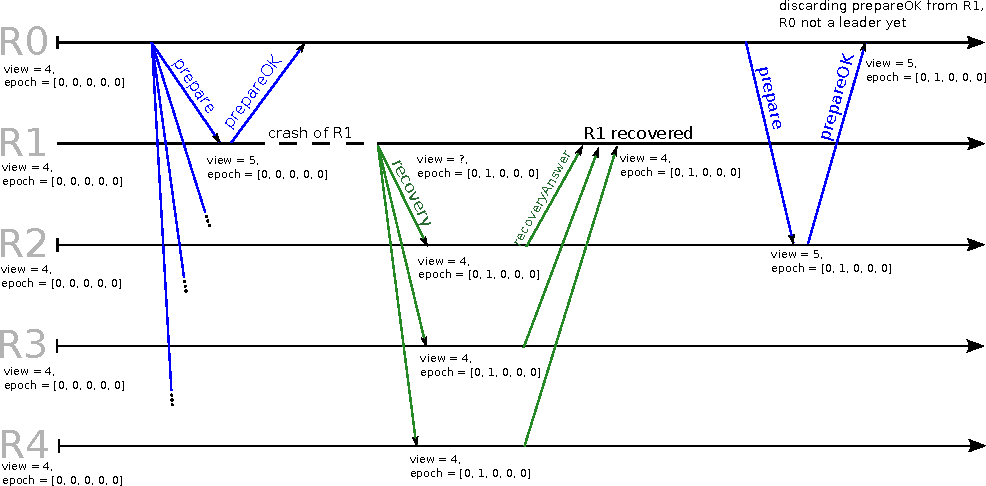
\includegraphics[keepaspectratio, width=0.9\textwidth]{epoch_recovery.pdf}
 \caption{Example of epoch-based recovery}
 \label{fig:epoch_based_recovery}
\end{figure}

\section{View-based recovery}
\label{sec:view_ss}

The next algorithm is view-based recovery. It has similar properties to epoch-based recovery. In every moment majority of processes is required to be correct but instead of using epoch numbers, the view number is written to table storage on every change. 

The pseudocode of this algorithm is presented below: 

\begin{algorithmic}[1]
  \INIT{}
    \STATE $log_p \leftarrow \bot$
    \STATE $view_p \leftarrow 0$
    \IF{$view_p \mod n = p$}
      \STATE $view_p \leftarrow view_p + 1$
    \ENDIF
    \STATE $state_p \leftarrow \bot$
    \STATE
    \IF{recovery after crash}
      \STATE $view_p \leftarrow$ last view number written to stable storage
      \IF{$view_p \mod n = p$}
        \STATE $view_p \leftarrow view_p + 1$
      \ENDIF
      \STATE send $<\recovery[], view_p>$ to all except $p$
      \STATE wait for $n-f <\recoveryAnswer[], view, highestId>$ messages including from primary of highest view received
      \STATE $view_p \leftarrow \max\{{ view \; \mathrm{received}}\}$
      \STATE download all instance up to $highestId$ from leader using catch-up module
    \ENDIF
    \STATE
    \STATE join Paxos protocol
  \ENDINIT

  \vspace{1em}
  \PROCEDURE{advanceView($view$)}
    \STATE write $view$ to stable storage
    \STATE $view_p \leftarrow view$
  \ENDPROC

  \vspace{1em}
  \UPON{receive $<\recovery[], view>$ from $q$}
    \IF{$q$ is primary of $view_p$}
      \STATE change to a higher view where $q$ is not primary
      \STATE wait until view change is complete
    \ENDIF
    \IF{$view > view_p$}
      \STATE advanceView(view)
    \ENDIF
    \STATE send $<\recoveryAnswer[], view_p, highestId_p>$ to $q$
  \ENDUPON
\end{algorithmic}

This algorithm makes synchronous write to stable storage on every view change. \linebreak If the network is stable and the leader does not crash, performance of the algorithm should be the same as in crash-stop model. If the view is changed often because of message loss or leader crash, the performance can decrease.

The recovery phase is quite similar to the epoch-based recovery. Recovering process is sending \recovery message to all and waits for majority of \recoveryAnswer to get $heighestId$ value from leader. Then catch-up mechanism is used to retrieve missing instances from correct processes. This algorithm is easier than based on epoch, because it doesn't introduce any changes in handling \prepareOK message.

\section{Comparison}

We presented 4 different algorithms implemented to JPaxos library. Each algorithm has different performance and fault tolerance. To choose the best algorithm for user service, we need to decide what fault tolerance and performance is required. In the table below, we present the comparison of all algorithms by comparing:
\begin{table}[h]
  \footnotesize
  \begin{tabular}{lccccc}
                        & Crash-stop & Full stable storage & View-based      & Epoch-based \vspace{0.2em} \\
    Decides by          & $2f+1$     & $2f+1$              & $2f+1$          & $2f+1$      \\
    Fault tolerance     & $2f+1$     & $f$                 & $2f+1$          & $2f+1$      \\
    Process can recover & no         & yes                 & yes             & yes         \\
    Stable storage use  & no         & per round           & per view change & on recovery \\
    Additional messages & ---        & ---                 & \recovery       & \recovery   \\
    State transfer      & no         & if needed           & yes             & yes         \\
    Increased msg size  & ---        & ---                 & ---             & \prepareOK by $n$\\
  \end{tabular}
  \caption{Comparison of recovery algorithms.}
  \scriptsize
\end{table}

\begin{figure}[h]
 \centering
 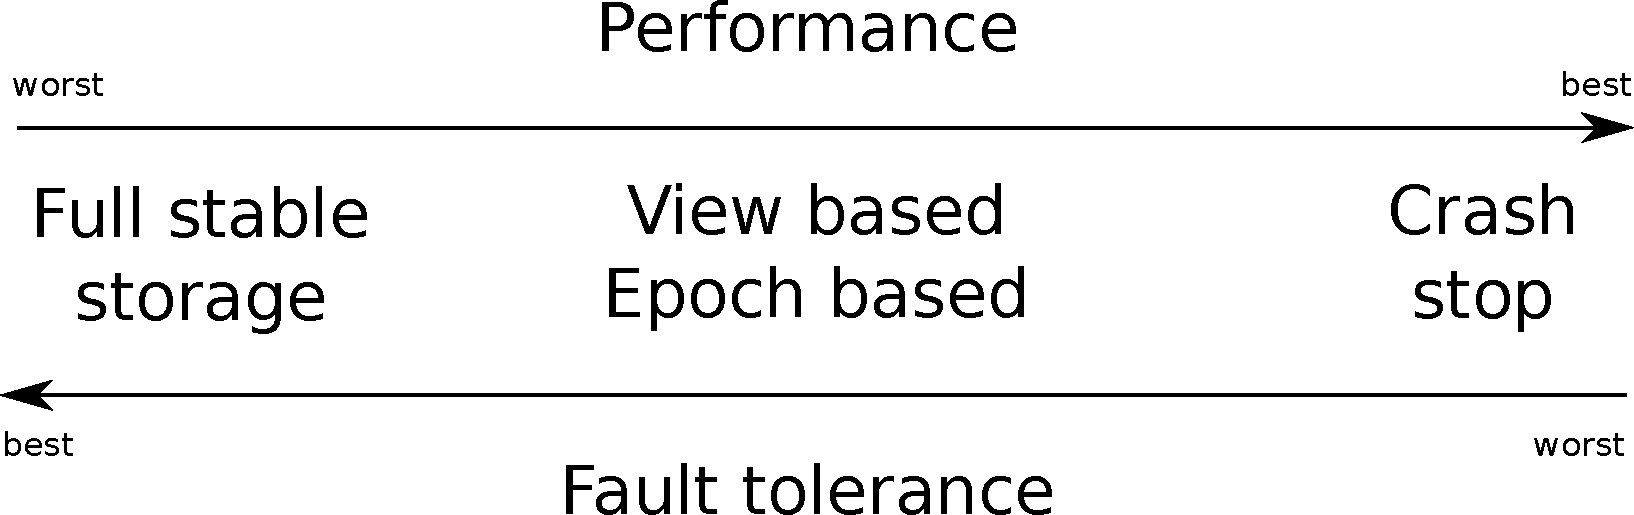
\includegraphics[keepaspectratio, width=0.75\textwidth]{recovery_algorithms.pdf}
 \caption{Comparison of recovery algorithms}
 \label{fig:recovery_algorithms}
\end{figure}

Crash recovery with full stable storage is an algorithm with the best fault tolerance because it tolerates catastrophic failures. However, to achieve that it makes a synchronous write to stable storage on every round (on every view and value change) what decreases the performance.

Crash stop doesn't provide any recovery (crashed processes will never be correct again) and all the time majority of processes have to be correct. However, no synchronous writes to stable storage are made so it provides the best performance.

The compromise between crash recovery with stable storage and crash stop are view-based and epoch-based recovery. They support recovery of crashed process and their performance should be close to crash-stop model. If service doesn't have to tolerate catastrophic failures, it is the best to use them in production environment.

Proofs of all algorithms presented in this chapter can be found in \cite{Nun10}. 
